\subsection{Funkcijos vidutinis greitis intervale}

\begin{equation}
    \frac{\Delta y}{\Delta x} = \frac{f(b) - f(a)}{b - a}
\end{equation}

\begin{equation}
    f(x) = 10x - 5, x \in [-5; 5] \\
    \frac{\Delta y}{\Delta x} = \frac{f(5) - f(-5)}{5 + 5} \\
    \frac{\Delta y}{\Delta x} = \frac{45 + 55}{10} = 10
\end{equation}

\subsection{Funkcijos greitis taške}

\begin{equation}
    \lim_{\Delta x \rightarrow 0} \frac{\Delta y}{\Delta x} = 
    \lim_{\Delta x \rightarrow 0} \frac{f(a + \Delta x) - f(a)}{\Delta x} = f^\prime(a)
\end{equation}

\begin{equation}
    f(x) = 5x^2 - 5, x = 5
\end{equation}
\begin{equation}
    \frac{f(5  + \Delta x) - f(5)}{\Delta x} = 
    \frac{5(5 + \Delta x)^2 - 5 - 125 + 5}{\Delta x} =
    \frac{5(25 + 2\Delta x + {(\Delta x)}^2) - 125}{\Delta x} =
\end{equation}
\begin{equation} 
    \frac{125 + 10\Delta x + 5{(\Delta x)}^2 - 125}{\Delta x} =
    \frac{10\Delta x + 5{(\Delta x)}^2}{\Delta x} =
    \frac{\Delta x (10 + 5\Delta x)}{\Delta x} = 10 + 5\Delta x
\end{equation}

\subsection{Funkcijos išvestinė funkcija}
\textit{Likusi šio skyriaus dalis aiškina kaip šito nenaudoti:}

\begin{equation}
    f^\prime(x) = \lim_{\Delta x \rightarrow 0} \frac{f(x + \Delta x) - f(x)}{\Delta x}
\end{equation}
\begin{equation}
    \lim_{\Delta x \rightarrow 0} \Delta x = 0
\end{equation}
\textit{Nesu tikras ar tikrai galima dauginti funkciją iš $\Delta x$\dots Turėtų būti galima\dots}
\begin{equation}
    y = f(x) = x^2 + 3
\end{equation}
\begin{equation}
     \lim_{\Delta x \rightarrow 0} \Delta x * f^\prime(x) = 
     \lim_{\Delta x \rightarrow 0} (f(x + \Delta x) - f(x)) = 
    \lim_{\Delta x \rightarrow 0} ((x + \Delta x)^2 + 3 - x^2 - 3) = 
\end{equation}
\begin{equation}
    \lim_{\Delta x \rightarrow 0} (x^2 + 2x\Delta x + (\Delta x)^2 + 3 - x^2 - 3) =
    \lim_{\Delta x \rightarrow 0} ((\Delta x)^2 + 2x\Delta x) = 
    \lim_{\Delta x \rightarrow 0} (\Delta x (\Delta x + 2x))
\end{equation}
\begin{equation}
    f(x) = \lim_{\Delta x \rightarrow 0} \frac{\Delta x (\Delta x + 2x)}{\Delta x} = 2x  
\end{equation}

\subsection{Liestinė}
\begin{equation}
    y = f^\prime(x_0)x + f(a_0) - af^\prime(x_0) =\underline{\ f^\prime(x_0)(x - x_0) + f(x_0)\ }
\end{equation}
\textit{Čia $x_0$ dažnai duodamas/surandamas.}

\textit{Funkcijos liestinė visada turės $y = kx + b$ pavidalą, todėl:}
\begin{equation}
    f^\prime(x_0) = \tg \alpha \\
    f^\prime(x_0) = k
\end{equation}

\subsection{Daugianario išvestinė}

\begin{equation}
    (af^\prime(x)) = af^\prime(x) \\
    a^\prime = 0 \Rightarrow {(x^a)}^\prime = a\,x^{a-1}
\end{equation}
\begin{equation}
    \frac{1}{x^n} = x^-n \\
    \sqrt[n]{x} = x^{\frac{1}{n}}
\end{equation}

\begin{equation}
    {(3x^7)}^\prime = 3 \cdot 7 x^6  = 21x^6 \\
    {(\sqrt{3 \cdot x})}^\prime = {(\sqrt{3} \cdot x^\frac{1}{2})}^\prime = 
    \sqrt{3} \cdot \frac{1}{2} x^{-\frac{1}{2}} = \dots = \frac{1}{2} \sqrt{\frac{3}{x}}
\end{equation}

\subsection{Kitos išvestinių formulės}

\begin{flalign}
    {(a^x)}^\prime = a^x \ln a,              \quad & (a > 0, a \ne 1) \\
    {(\log_a x)}^\prime = \frac{1}{x \ln a}, \quad & (a > 0, a \ne 1) \\
    {(\sin x)}^\prime = \cos x;              \quad & \qquad {(\cos x)}^\prime = -\sin x \\
    {(\tg x)}^\prime = \frac{1}{\cos^2 x};   \quad & \qquad {(\ctg x)}^\prime = -\frac{1}{\sin^2 x} \\
    {(f(x) \cdot g(x))}^\prime &= f^\prime(x) \cdot g(x) + f(x) \cdot g^\prime{x} \\
    {\Bigl(\frac{f(x)}{g(x)}\Bigr)}^\prime &= \frac{f^\prime(x)\cdot g(x) - f(x)\cdot g^\prime{x}}{g^2(x)} \\
    {\Bigl(f(g(x))\Bigr)}^\prime &= f^\prime(g(x)) \cdot g^\prime(x)
\end{flalign}

\subsubsection{Daugiau}
\begin{equation}
    \ln x = \log_e x \quad \Rightarrow \quad (e^x)^\prime = e^x, \qquad (\ln x)^\prime = \frac{1}{x}
\end{equation}

\subsection{Funkcijos reikšmių kitimas}

\textit{Beje, išvestinės nedraugauja su \href{https://lt.wikipedia.org/wiki/Tolydi_funkcija}{netolydžiomis(nutrūkstančiomis/šokinėjančiomis) funkcijomis}, nes, pavyzdžiui: tokios funkcijos gali turėti ir teigiamas, ir neigiamas reikšmes, bet niekad nekirsti OX (abscisių) ašies.}

\begin{align}
    f^\prime(x) = 0 \quad &\Rightarrow \quad \text{funkcijos reikšmė -- pastovi} \\
    f^\prime(x) > 0 \quad &\Rightarrow \quad \text{funkcijos reikšmė -- didėja} \\
    f^\prime(x) < 0 \quad &\Rightarrow \quad \text{funkcijos reikšmė -- mažėja} \\
\end{align}

Ekstremumo taškai -- minimumo ir maksimumo taškai.
Minimumo taškas -- pastovumo taškas kai mažėjanti funkcijos dalis pradės augti.
Maksimumo taškas turi atvirkščią apibrėžimą minimumo taškui.

Beje, jei funkcija yra uždarame intervale, intervalo kraštai veikia taip pat kaip ekstremumo taškai. 

\begin{equation}
    f(x) = 2x^3 - x^2 \quad
    f^\prime(x) = 6x^2 - 2x 
\end{equation}
\begin{equation}
    6x^2 - 2x = 0 \quad
    x(6x - 2) = 0 \quad
    x = 0 \arba x = 1/3 
\end{equation}
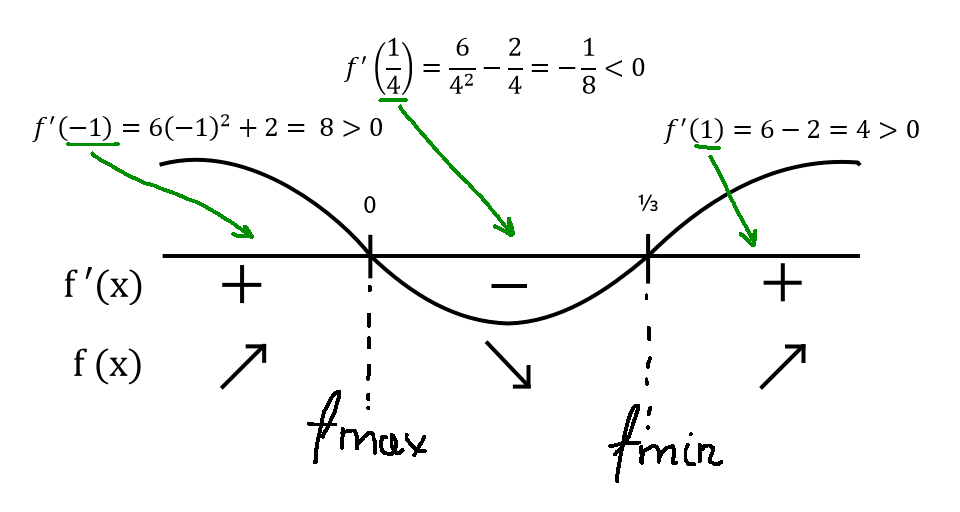
\includegraphics[max width=\textwidth]{assets/derivatives_extreme_points.png}

\subsection{Funkcijų tirimas}

\begin{enumerate}
    \item Apibrėžimo sritis:    \quad $D_f$
    \item Funkcijos lyginumas:  \quad $f(x) = f(-x),\ |f(x)| = |f(-x)|,\ f(x) \ne f(-x)$
    \item Kur kerta OX ašį:     \quad $f(x) = 0$
    \item Kur kerta OY ašį:     \quad $f(0) = y$
    \item Kritiniai taškai:     \quad $f^\prime(x) = 0$
    \item Reikšmės kitimo intervalai: \quad $f^\prime(x) \lessgtr 0$
    \item Ekstremumo taškai:    \quad $f_{min}, f_{max}; f^\prime(x) = 0 \Rightarrow f(x) = y$
\end{enumerate}

\subsection{Daugiau}

Tekstiniai uždaviniai, kurie reikalauja išvestinių dažnai prašo surasti su kokiais parametrais, rezultatas bus dižiausias/mažiausias. Be to, šie uždaviniai \textbf{dažnai} neduos užtektinai dydžių, kad būtų galima apkaičiuoti, koks dalykas yra pateiktu atveju.  

